%%%%%%%%%%%%%%%%%%%%%%%%%%%%%%%%%%%%%%%%%%%%%%%%%%%%%%%%%%
%%
%%  LOD-L2.tex
%%  Lecture 2: Diffeology, the Axiomatic
%%
%%%%%%%%%%%%%%%%%%%%%%%%%%%%%%%%%%%%%%%%%%%%%%%%%%%%%%%%%%

\chapter*{\S L2. Diffeology, the Axiomatic}
\setcounter{footnote}{0}

%%%%%%%%%%%%%%%%%%%%%%%%%%%%%%%%%%%%%%%%%%%%%%%%%%%%%%%%%%
%%
%% MARK: Abstract
%%
%%%%%%%%%%%%%%%%%%%%%%%%%%%%%%%%%%%%%%%%%%%%%%%%%%%%%%%%%%
\begin{abstract}
  In this lecture we will look at the short axiomatic that founds diffeology.
  It describes the basic set-theoretic constructions of the theory and gives a few examples.
\end{abstract}

%%%%%%%%%%%%%%%%%%%%%%%%%%%%%%%%%%%%%%%%%%%%%%%%%%%%%%%%%%
%%
%% MARK: Introduction
%%
%%%%%%%%%%%%%%%%%%%%%%%%%%%%%%%%%%%%%%%%%%%%%%%%%%%%%%%%%%

Diffeologies are defined on arbitrary sets without any preexisting structure,
neither topology nor anything else.
That is important enough to be underlined and remembered.
Diffeology is based on the notion of parametrizations,
and will consist of declaring which parametrizations in a set will be regarded as smooth,
provided that a small set of axioms is satisfied.
Then,
the development of diffeology will consist of transferring,
through these specific parametrizations,
significative properties and constructions \emph{a priori} defined in the category of smooth domains,
such as homotopy groups,
fiber bundles,
differential forms\dots for example.

%%%%%%%%%%%%%%%%%%%%%%%%%%%%%%%%%%%%%%%%%%%%%%%%%%%%%%%%%%
%%
%% MARK:  What is a Diffeology
%%
%%%%%%%%%%%%%%%%%%%%%%%%%%%%%%%%%%%%%%%%%%%%%%%%%%%%%%%%%%

\section{What is a diffeology?}

The theory of diffeology begins with the idea of parametrization.
The first step in this direction was taken by K.T.~Chen in his paper on ``Iterated Path Integrals'' \cite{Che77},
but the parametrizations were defined on convex subsets of Euclidean domains.
In 1980,
in his paper on ``Groupes diff\'erentiels'' \cite{Sou80},
J.M.~Souriau keeps the same axiomatic but with parametrizations defined on Euclidean domains,
open subsets of Euclidean spaces.
That is what founds today's diffeology:

\begin{Article}{Parametrizations.}
  We call \emph{parametrization} in a set $X$ any map $P \colon U \to X$ where $U$ is some Euclidean domain,
  that is,
  any open subset of a Euclidean space.
  If we want to be specific,
  we say that $P$ is an \emph{$n$-parametrization} when $U$ is an open subset of $\RR^n$.
  The set of all parametrizations in $X$ is denoted by
  $$%
    \Params(X) = \{ P \colon U \to X \mid U \in \Domains(\RR^n), n \in \RR \}
    $$%
\end{Article}
%
\uline{Note that} there is no condition of injectivity on $P$,
and as we said,
neither any topology precondition on $X$ a priori.

\begin{Article}{Diffeology.}
  A \emph{diffeology} on a set $X$ is any subset
  $$%
    \cD \subset \Params(X)
    $$%
  that satisfies the following axioms:
  \begin{enumerate}
    \item[1.] \emph{Covering}: $\cD$ contains the constant parametrizations.
    \item[2.] \emph{Locality}: Let $P \colon U \to X$ be a parametrization.
    If,
    for all $r \in U$,
    there is an open neighbourhood $V$ of $r$ such that $P \restriction V \in \cD$,
    then $P \in \cD$.
    \item[3.] \emph{Smooth compatibility}: For all $P \colon U \to X$ in $\cD$,
    for all $F \in \Cinfty(V,U)$,
    where $V$ is a Euclidean domain,
    $P \circ F \in \cD$.
  \end{enumerate}
  A space equipped with a diffeology is called a \emph{diffeological space}.
  The elements of the diffeology $\cD$ of a diffeological space $X$ are called the \emph{plots} of (or in) the space.%
  \footnote{There is a discussion about diffeology as a sheaf theory in \cite[Annex]{Igl87}.
  But we do not develop this formal point of view in general,
  because the purpose of diffeology is to minimize the technical tools in favour of a direct,
  more geometrical,
  intuition.}
\end{Article}

\begin{Article}{Note.}{}
  Formally,
  a diffeological space is a pair $(X,\cD)$ where $X$ is the underlying set and $\cD$ the chosen diffeology,
  but we generally use a single letter to make the reading lighter.
  For example,
  we can use the letter $\cX$ for the pair $(X,\cD)$,
  or anything else suggestive.
\end{Article}

\begin{Article}{Example: smooth diffeology on $\RR^n$.}
  The first and foremost examples of diffeological spaces are the Euclidean domains.
  The plots of a domain $\cO$ are all the smooth parametrizations $F \colon U \to \cO$,
  where $U$ is any other domain,
  of any dimension.
  We call this diffeology the \emph{smooth diffeology},
  or the \emph{standard diffeology}.
  It is clear that the three axioms are satisfied.
  They have been chosen exactly because they are the fundamental properties which we want to replicate on sets,
  to define a \emph{smooth structure}.
  Note that this is not the only way to imagine smooth structure on sets.
  We may compare diffeology with other approaches in the future.
\end{Article}

%%%%%%%%%%%%%%%%%%%%%%%%%%%%%%%%%%%%%%%%%%%%%%%%%%%%%%%%%%
%%
%% MARK:  Category Diffeology
%%
%%%%%%%%%%%%%%%%%%%%%%%%%%%%%%%%%%%%%%%%%%%%%%%%%%%%%%%%%%
\section{Category \{Diffeology\}}

\begin{Article}{Smooth maps.}
  After defining the structure of diffeological space,
  the main constituent in diffeology is the notion of \emph{smooth map}.
  Let $X$ and $X'$ be two diffeological spaces.
  A map $f \colon X \to X'$ is said to be smooth if (and only if) the composite with any plot in $X$ is a plot in $X'$,
  which can be summarized by
  $$%
    f \circ \cD\subset \cD',
    $$%
  where $\cD$ and $\cD'$ denote the respective diffeologies.
  The set of smooth maps from $X$ to $X'$ is denoted by%
  \footnote{$\Maps(X,X')$ denotes the set of all maps from $X$ to $X'$.}
  $$%
    \Cinfty(X,X') = \{f \in \Maps(X,X') \mid f \circ P \in \cD', \ \forall P \in \cD \}.
    $$%
\end{Article}

\begin{Article}{Example: smooth parametrizations.}
  The plots of a diffeology are the first examples of smooth maps.
  Indeed,
  let $P \colon U \to X$ be a plot of $X$,
  let $F \colon V \to U$ be a plot of the smooth diffeology on the domain $U$,
  that is $F \in \Cinfty(V,U)$.
  Then,
  the composite $P \circ F$ is a plot of $X$,
  that is the third axiom of diffeology,
  the ``smooth compatibility''.
  Therefore,
  $$%
    \Cinfty(U,X) = \{ P \in \cD \mid \Domain(P) = U \}.
    $$%
  In particular,
  for the domains $U$ and $V$,
  the notation $\Cinfty(U,V)$ is understood in the usual sense and in the diffeological sense coincide.
  Hence,
  there is no need to introduce a special notation to denote the plots of a diffeological space.
\end{Article}

\begin{Article}{Category \{Diffeology\}.}
  Consider $X$,
  $X'$ and $X''$ be three diffeological spaces,
  with diffeologies $\cD$,
  $\cD'$ and $\cD''$.
  Let $f \in \Cinfty(X,X')$ and $f' \in \Cinfty(X',X'')$,
  then $f' \circ f \in \Cinfty(X,X'')$.
  Thus,
  diffeological spaces,
  together with smooth maps,
  define a category we write \{Diffeology\}.
  
  The isomorphisms of this category are called \emph{diffeomorphisms},
  they are bijective maps,
  smooth as well as their inverse.
  In the case of a diffeomorphism $f \circ \cD = \cD'$.
  The set of diffeomorphisms from $X$ to $X'$ is denoted by $\Diff(X,X')$.
\end{Article}

\begin{Article}{Remark.}{}
  \{Euclidean Domains\} is a full subcategory of \{Diffeology\},
  which is a strict extension of it on sets.
  We could call such extensions ``smooth categories'',
  but that is just to identify the general context of the theory.
\end{Article}

Pick,
for example,
the smooth $\RR^2$:
we have a diffeology on $\Torus^2 = \RR^2/\ZZ^2$ by lifting locally the parametrizations in $\RR^2$.
That is,
a plot of $\Torus^2$ will be a parametrization $P \colon r \mapsto (z_r,z'_r)$ such that,
for every point in the domain of $P$,
there exist two smooth parametrizations $\theta$ and $\theta'$, in $\RR$,
defined in the neighbourhood of this point,
with $(z_r,z'_r)= (e^{2i\pi\theta(r)},e^{2i\pi\theta'(r)})$,
that is,
the usual diffeology that makes $\Torus^2$ the manifold we know.

That procedure can be extended naturally to the quotient $\Torus_\alpha = \RR/(\ZZ + \alpha \ZZ)$,
where $\alpha$ is some number.
Indeed,
a parametrization $P \colon r \mapsto \tau_r$ in $\Torus_\alpha$ is a plot if there exists locally,
in the neighbourhood of every point in the domain of $P$,
a parametrization $r \mapsto t_r$,
such that $\tau_r= \Class(t_r)$,
with $\Class : \RR \to \Torus_\alpha$ the projection.

This is exactly the diffeology we are considering when we talk about the irrational torus.
This construction of diffeologies by \emph{pushforward} is actually one of the fundamental constructions of the theory,
and for that,
we need to introduce an important property of the set of diffeologies of a set.

%%%%%%%%%%%%%%%%%%%%%%%%%%%%%%%%%%%%%%%%%%%%%%%%%%%%%%%%%%
%%
%% MARK:  Order in Diffeology
%%
%%%%%%%%%%%%%%%%%%%%%%%%%%%%%%%%%%%%%%%%%%%%%%%%%%%%%%%%%%
\section{Order in diffeology}

\begin{Article}{Comparing diffeologies.}
  Inclusion defines a partial order in diffeology,
  called \emph{fineness}.
  If $\cD$ and $\cD'$ are two diffeologies on a set $X$,
  one says that $\cD$ is \emph{finer} than $\cD'$ if $\cD \subset \cD'$.
  We denote by
  $$%
    \cD \preceq \cD'.
    $$%
  \begin{figure}[htb]
    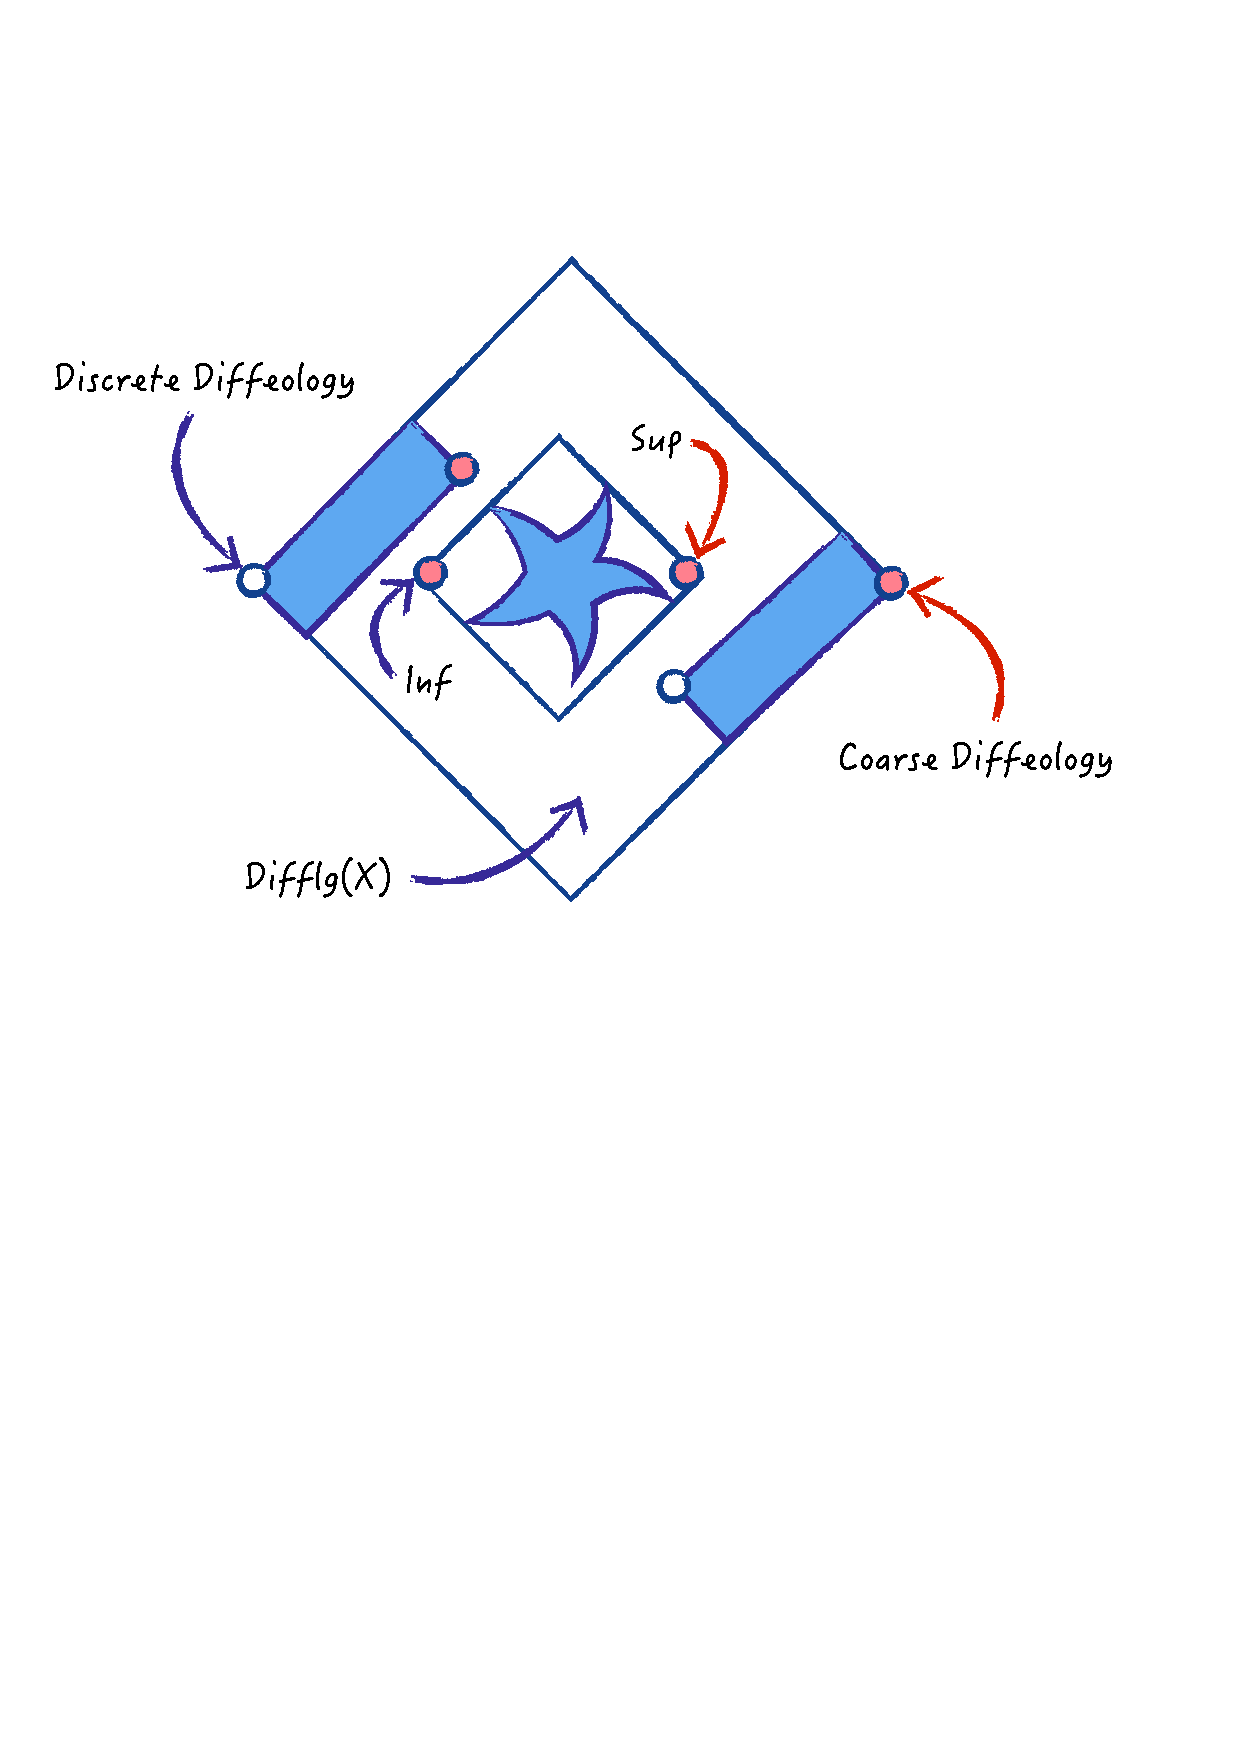
\includegraphics[width=1.0\textwidth]{Figures/Comparing-diffeologies.pdf}
    \caption{Comparing Diffeologies.}
    \label{Comparing-diffeologies.}
  \end{figure}
  We say also that $\cD'$ is \emph{coarser} than $\cD$.
  Every set has two extreme diffeologies:
  \begin{enumerate}
    \item The \emph{discrete diffeology} where plots are only local constant parametrizations is the finest.
    \item The \emph{coarse diffeology} where plots are all the parametrizations is the coarsest.
  \end{enumerate}
\end{Article}

\begin{Article}{Infimum and supremum.}
  Diffeologies are stable by intersection.
  Any family $(\cD_i)_{i \in \cI}$ of diffeologies on a set $X$ has an \emph{infimum},
  it is the intersection:
  $$%
    \inf(\cD_i)_{i \in \cI} = \bigcap_{i \in \cI} \cD_i.
    $$%
  It is the coarsest diffeology which is contained in every element of the family $(\cD_i)_{i \in \cI}$.
  
  The family $(\cD_i)_{i \in \cI}$ has also a \emph{supremum},
  it is the finest diffeology containing every element of the family:
  $$%
    \Sup(\cD_i)_{i \in \cI} = \inf\{\cD' \in \Difflg(X) \mid \forall i \in \cI, \cD_i \subset \cD' \}
    $$%
  where \emph{$\Difflg(X)$} denotes the set of all diffeologies on the set $X$.
  
  This partial order,
  fineness,
  makes the set of diffeologies on a set $X$,
  a \emph{lattice}.
  That is,
  a set such that every subset of diffeologies has an infimum and a supremum.
  
  As usual,
  if the infimum of a family belongs to the family,
  then it is called a \emph{minimum};
  and if the supremum belongs to the family,
  then it is called the \emph{maximum}.
  
  This property of being a lattice is very useful in defining diffeologies by means of properties.
  We shall see that most of diffeologies are the finest or coarsest diffeologies such that some property is satisfied.
  Because minima and maxima are always distinguished elements in a set when they exist.
  The following examples will illustrate the point.
\end{Article}

%%%%%%%%%%%%%%%%%%%%%%%%%%%%%%%%%%%%%%%%%%%%%%%%%%%%%%%%%%
%%
%% MARK:  Pushing and Pulling Diffeology
%%
%%%%%%%%%%%%%%%%%%%%%%%%%%%%%%%%%%%%%%%%%%%%%%%%%%%%%%%%%%
\section{Pushing and pulling diffeology}


\begin{Article}{Pushing forward diffeologies.}
  Let $f \colon X \to X'$ be a map,
  and let $X$ be a diffeological space,
  with diffeology $\cD$.
  Then,
  there exists a finest diffeology on $X'$ such that $f$ is smooth.
  It is called the \emph{pushforward} of the diffeology of $X$.
  We denote it by $f_*(\cD)$.
  
  If $f$ is surjective,
  its plots are the parametrizations $P'$ in $X'$ that can be written $\Sup_i f \circ P_i$,
  where the $P_i$ are plots of $X$ such that the $f \circ P_i$ are compatible,
  that is,
  coincide on the intersection of their domains,
  and $\Sup$ denotes the smallest common extension of the family $\{f\circ P_i\}_{i\in \cI}$.
  Formally speaking,
  a parametrization $P' \colon U \to X$ belongs to $f_*(\cD)$,
  if (and only if) there exists a family $(P_i)_{i \in \cI}$ of plots of $X$,
  $P_i \in \cD$,
  defined on an open covering $(U_i)_{i \in \cI}$ of $U$,
  such that $f \circ P_i = P' \restriction_{U_i}$.
  $$%
    f_*(\cD) = \{ P' \in \Params(X') \mid \exists P_i \in \cD, i \in \cI, P' = \Sup_i(f\circ P_i) \}.
    $$%
  \uline{It is equivalent} to say that for all $r \in U$ there exists an open neighbourhood $V$ and a plot $Q$ in $X$,
  such that $P \restriction V = f \circ Q$.
\end{Article}

\begin{Article}{Subductions.}
  Let $\pi \colon X \to X'$ be a map between diffeological spaces.
  We say that $\pi$ is a \emph{subduction} if (and only if)
  
  \begin{enumerate}
    \item The map $\pi$ is surjective.
    \item The pushforward of the diffeology of $X$ coincides with the diffeology of $X'$.
  \end{enumerate}
  
  We can check that the composite of two subductions is again a subduction,
  that makes the subcategory \{Subductions\}.
\end{Article}

Let's talk about quotients.

\begin{Article}{What a quotient is and where does it live.}
  There is sometimes an ambiguity about the construction of quotient sets that needs to be addressed once and for all.
  They are too often identified with some sets of representatives in a way that can be regarded as arbitrary.
  Let us begin with a set $X$ and an \emph{equivalence relation} $\sim$ on $X$,
  that is,
  a binary relation which is reflexive,
  symmetric and transitive.
  Let $x \in X$,
  the \emph{equivalence class} $\Class(x)$ of $x$ is by definition the subset
  $$%
    \Class(x) = \{ x' \mid x' \sim x \} \subset X.
    $$%
  It lives then naturally in the \emph{powerset}
  $$%
    \Class(x) \in \fP(X) = \{ A \mid A \subset X\},
    $$%
  set of all the subsets of $X$.
  The quotient set $Q$ of $X$ by $\sim$,
  denoted generally by $X/\!\!\sim$,
  can always be regarded as a subset of $\fP(X)$:
  $$%
    Q = \{ \Class(x) \mid x \in X \} \subset \fP(X).
    $$%
  The \emph{canonical projection} $\Class$ is then the application
  $$%
    \Class \colon X \to \fP(X)
    \quad \text{with} \quad
    X/\!\!\sim \ = \Class(X).
    $$%
  When it comes to quotient space in these lectures,
  it is always the way we look at it.
\end{Article}

\begin{Article}{Quotient spaces.}
  Let $X$ be a diffeological space and let $\sim$ be an equivalence relation on $X$.
  Let $Q = X/\!\!\sim$ be the quotient set.
  The pushforward $\Class_*(\cD)$ on  $Q$ of the diffeology of $X$,
  by the canonical projection,
  is called the \emph{quotient diffeology}.
  Equipped with the quotient diffeology,
  $Q$ is called the \emph{quotient space} of $X$ by $\sim$.
  
  This is the first important property of the category \{Diffeology\},
  \uline{it is closed by quotient},
  and we shall see not trivially closed.
  
  \uline{Note that} considering the quotient $Q = X/\!\!\sim$ for what it is,
  as described above,
  does not prevent us to identify it with some smooth representative $\cQ$,
  according to the diagram where $\Class$ and $\pi$ are two subductions and $f$ a bijection,
  and therefore a diffeomorphism.
  %
  \begin{center}
    \begin{tikzcd}[column sep=small, row sep=large, every label/.append style = {font = \small}]
      & X \arrow[dl, swap, "\Class"] \arrow[dr, "\pi"] & \\
      Q \arrow[rr, swap, "f"] &  & \cQ
    \end{tikzcd}
  \end{center}
\end{Article}
%
\begin{Article}{Pulling back diffeologies.}
  Let $f \colon X \to X'$ be a map,
  and let $X'$ be a diffeological space with diffeology $\cD'$.
  Then,
  there exists a coarsest diffeology on $X$ such that $f$ is smooth.
  It is called the \emph{pullback} of the diffeology of $X'$.
  We denote it by $f^*(\cD')$.
  Its plots are the parametrizations $P$ in $X$ such that $f \circ P$ is a plot of $X'$.
  $$%
    f^*(\cD') = \{ P \in \Params(X) \mid f \circ P \in \cD' \}.
    $$%
\end{Article}

\begin{Article}{Inductions.}
  Let $X$ and $X'$ be two diffeological spaces and $f \colon X \to X'$ be a map.
  We say that $f$ is an induction if (and only if):
  %   The map $f$ is injective and the pullback $f^*(\cD')$ of the diffeology of $X'$ coincides with the diffeology $\cD$ of $X$.\n
  \begin{enumerate}
    \item The map $f$ is injective.
    \item The pullback $f^*(\cD')$ of the diffeology of $X'$ coincides with the diffeology $\cD$ of $X$.
  \end{enumerate}
\end{Article}

\begin{Article}{Subset diffeology.}
  Pulling back diffeologies gives to any subset $A \subset X$,
  where $X$ is a diffeological space,
  a \emph{subset diffeology} $j^*(\cD)$,
  where $j \colon A \to X$ is the inclusion and $\cD$ is the diffeology of $X$.
  A subset equipped with the subset diffeology is called a \emph{diffeological subspace}.
  Plots of the subset diffeology are simply plots of $X$ taking their values in the subset $A$.
  
  This is a second important property of the category \{Diffeology\},
  \uline{it is closed by inclusion}.
\end{Article}

\begin{Article}{Discrete subspaces.}
  We have defined \emph{discrete diffeological spaces} as diffeological spaces equipped with the discrete diffeology.
  That is,
  the diffeology consisting in locally constant parametrization.
  It happens that subspaces of diffeological spaces inherit the discrete diffeology.
  
  The \smuline{prime example} of a discrete subset in diffeology is probably $\QQ \subset \RR$.
  This corresponds perfectly to what we understand intuitively to be discrete.
  But we have to be careful because discrete in diffeology does not coincide always with discrete in topology,
  in particular for $\QQ$ in $\RR$ that topologists do not consider as discrete,
  which is a little bit exaggerated.
  However,
  it is always preferable to specify in which sense we are using the word ``discrete'' when in doubt,
  to avoid any confusion with topologists.
\end{Article}

\begin{proof}
  Consider a plot $P \colon U \to \RR$ but with values in $\QQ$.
  Let $r, r' \in U$ and $\gamma \colon t \mapsto P(tr' +(1-t)r )$,
  defined on a small open neighbourhood of $[0,1]$.
  Then,
  $\gamma$ is a plot in $\RR$ and therefore continuous.
  Let $q = \gamma(0) = P(r)$ and $q' = \gamma(1) = P(r')$,
  by hypothesis $q,q' \in \QQ$.
  Since $\gamma$ is continuous,
  according to the \emph{intermediate value theorem},%
  \footnote{\url{https://en.wikipedia.org/wiki/Intermediate_value_theorem}.}
  $\gamma$ takes every value between $q$ and $q'$.
  If $q \neq q'$, there exists always an irrational number in between,
  which cannot be because $P$ takes its values only in $\QQ$.
  Therefore $\gamma(0) = \gamma(1)$,
  that is,
  $P(r) = P(r')$.
  The plot $P$ is then locally constant since it will be constant on every small ball around every $r \in U$.
\end{proof}

\begin{Article}{Example: the circle.}
  Let $\Sph^1$ be the circle,
  defined by
  $$%
    \Sph^1 = \{ (x,y) \in \RR^2 \mid x^2 + y^2 = 1 \}.
    $$%
  It is equivalent to the set $\U(1)$ of complex numbers of modulus $1$,
  $z = x+iy \in \U(1)$ means%
  \footnote{$\bar z$ or $z^*$ denote the conjugate $x-iy$ of $z = x +iy$.}
  $\bar z z = x^2 + y^2 =1$.
  The plots of $\Sph^1$,
  as a diffeological subspace of $\RR^2$,
  are just the pairs $r \mapsto (x(r), y(r))$ of smooth real functions defined on some Euclidean domain $U$,
  such that for all $r$ in $U$,
  $x(r)^2 + y(r)^2 = 1$.
  In particular,
  for $r = \theta \in \RR$:
  
  \textbf{Proposition.}{\itshape The projection,
  from $\RR$ to $\Sph^1$,
  $$%
    \pi \colon \theta \mapsto (\cos(\theta), \sin(\theta))
    $$%
  is a subduction.}
  
  Indeed,
  For any $\theta$,
  one of the derivatives $x'(\theta) = -\sin(\theta)$ or $y'(\theta) = \cos(\theta)$ does not vanish,
  since $x'(\theta)^2 + y'(\theta)^2 = 1$.
  Assume that $x'(\theta_0) \neq 0$,
  then according to the inverse function theorem,%
  \footnote{\url{https://en.wikipedia.org/wiki/Inverse_function_theorem}.}
  there exists a small interval $\cI$ centered at $\theta_0$ such that $\pphi = \cos \restriction \cI$ is a diffeomorphism onto its image,
  an open interval that we denote by $\cJ = \cos(\cI)$.
  So,
  let $r \mapsto (x(r), y(r))$ be a plot in $\Sph^1$ and assume that $x(r_0) = \cos(\theta_0)$ and $\sin(\theta_0) \neq 0$.
  The preimage $\cO = x^{-1}(\cJ)$ is an open subset in $U$,
  since $r \mapsto x(r)$ is smooth.
  
  \begin{figure}[htb]
    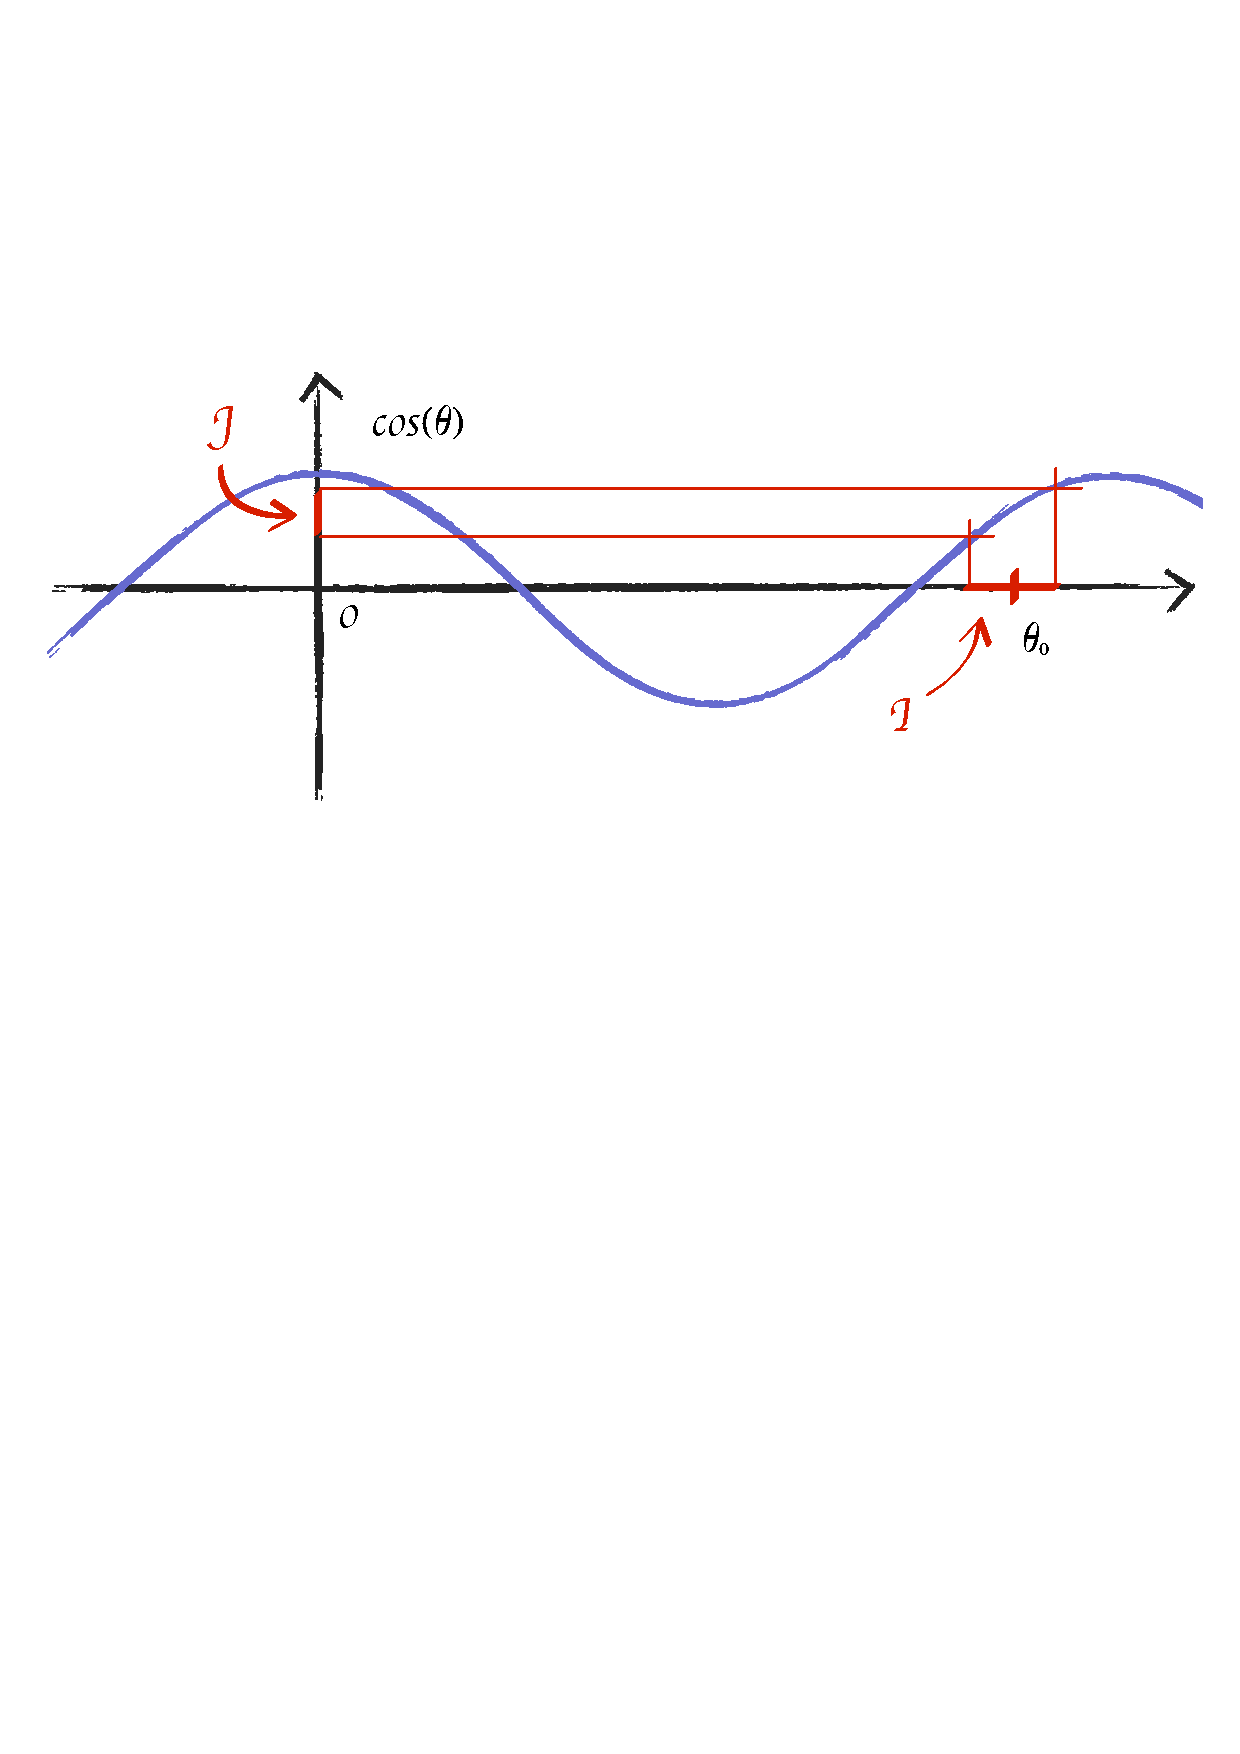
\includegraphics[width=0.75\textwidth]{Figures/Cos-theta.pdf}
    \caption{Function Cosinus.}
    \label{Function-Cosinus.}
  \end{figure}
  
  Then,
  let $\theta(r) = \pphi^{-1}(x(r))$,
  defined on $\cO$,
  and for all $r \in \cO$,
  $x(r) = \cos(\theta(r))$ and $y(r) = \sin(\theta(r))$.
  The map $r \mapsto \theta(r)$ is a \emph{local lifting},
  along the projection $\pi$,
  of the plot $r \mapsto (x(r), y(r))$.
  
  There exists then a bijection $f \colon \RR/2\pi\ZZ \to \Sph^1$
  $$%
    f(\Class(x))) = (\cos(x),\sin(x)),
    $$%
  and since $\pi \colon x \mapsto (\cos(x), \sin(x))$ is a subduction,
  $f$ is a diffeomorphism satisfying $f \circ \Class = \pi$,
  and therefore $\Sph^1$ is a smooth representative of $\RR/2\pi\ZZ$.
  
  On the other hand,
  we can define also
  $$%
    \sigma \colon x \mapsto {x \over 2\pi} - \left[{x \over 2\pi}\right],
    $$%
  where the bracket denotes the integer part.
  Then $\sigma(x) = \sigma(x')$ if and only if $x' = x + 2\pi k$,
  with $k \in \ZZ$.
  Set theoretically,
  the interval $\LeftClosedInterval{0,2\pi} = \sigma(\RR) \subset \RR$ represents $\RR/2\pi\ZZ$,
  but equipped with the subset diffeology,
  $\sigma$ is discontinuous and it cannot be a smooth representation of the quotient $\RR/2\pi\ZZ$.
  \begin{figure}[ht]
    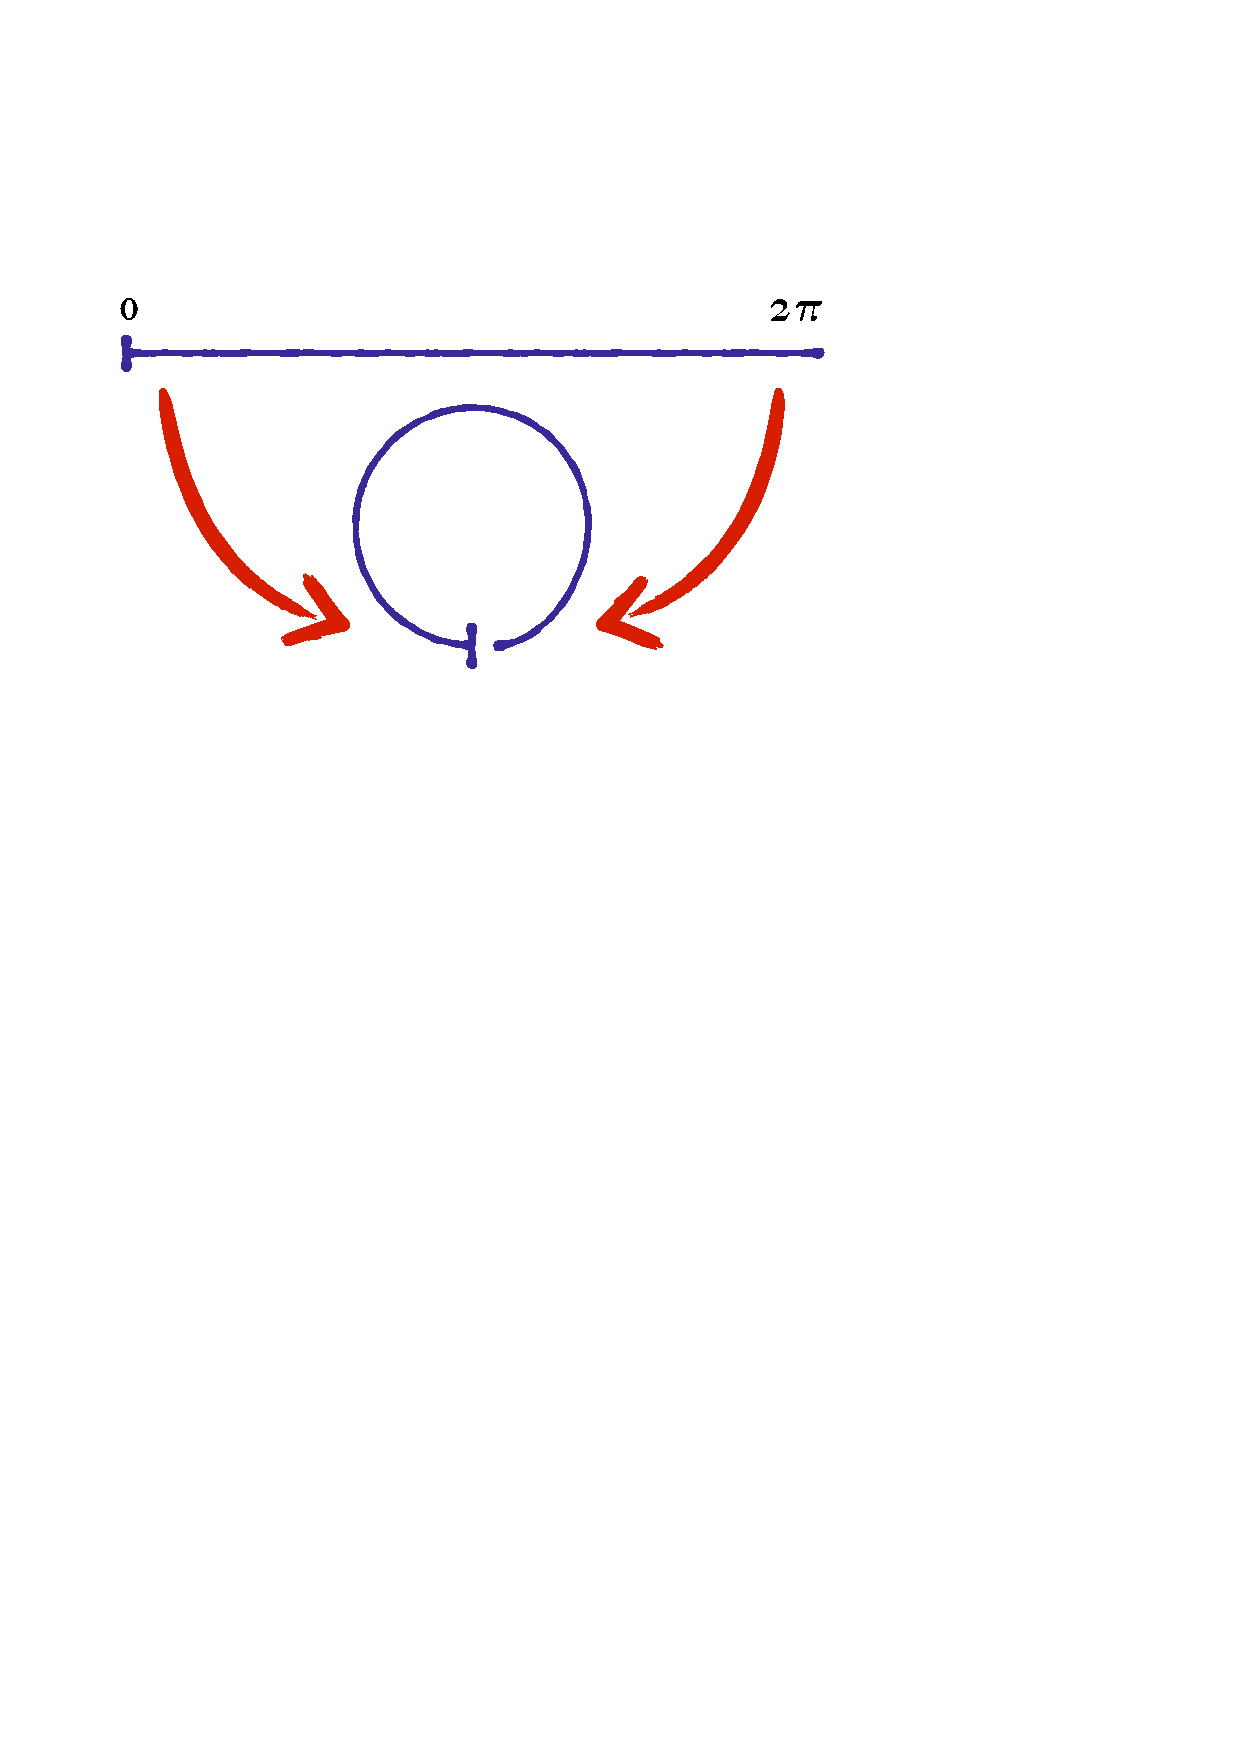
\includegraphics[width=0.5\textwidth]{Figures/Cut-circle.pdf}
    \vspace{-0.5\baselineskip}
    \caption{Closing the circle by push forward.}
    \label{Cut-circle}
  \end{figure}
  Of course we can push forward the smooth diffeology of $\RR$ onto the segment $\LeftClosedInterval{0,2\pi}$,
  but that would consist of gluing the end of the interval near $2\pi$ to the origin $0$,
  and so to reconstruct the circle as shown in Figure \ref{Cut-circle}.
\end{Article}

\begin{Article}{Strict maps.}
  The last example of the projection $\pi \colon \theta \mapsto (\cos(\theta),$%
  \linebreak
  $\sin(\theta))$,
  from $\RR$ to $\Sph^1 \subset \RR^2$ suggests the definition of a new kind of map,
  the \emph{strict maps}.
  
  Every map $f \colon X \to Y$ defines the following commutative diagram
  \begin{center}
    \begin{tikzcd}[column sep=small, row sep=large, every label/.append style = {font = \small}]
      X \arrow[r, "f"] \arrow[d, swap, "class"] &  X'    \\
      X/f \arrow[r, swap, "\pphi"] & f(X) \arrow[u, swap, "j"]
    \end{tikzcd}
  \end{center}
  where
  \begin{enumerate}
    \item $X/f$ denotes the quotient by the relation $f(x) = f(x')$.
    \item The map $j \colon f(X) \to X'$ is the inclusion.
    \item The map $\pphi \colon X/f \to f(X)$ is defined by $\pphi(\Class(x)) = f(x)$.
  \end{enumerate}
  Let now $X$ and $X'$ be two diffeological spaces:
  
  We say that $f$ is \emph{strict} if $\pphi$ is a diffeomorphism when $X/f$ is equipped with the quotient diffeology and $f(X)$ with the subset diffeology.
  
  In particular,
  the map $\pi$ above is strict.
  Strict maps realize quotient as subset of other diffeological spaces.
\end{Article}

%%%%%%%%%%%%%%%%%%%%%%%%%%%%%%%%%%%%%%%%%%%%%%%%%%%%%%%%%%
%%
%% MARK:  Making Sum of Diffeologies
%%
%%%%%%%%%%%%%%%%%%%%%%%%%%%%%%%%%%%%%%%%%%%%%%%%%%%%%%%%%%
\section{Making sum of diffeologies}

\begin{Article}{Direct sum diffeology.}
  Consider a family $(X_i)_{i \in \cI}$ of diffeological spaces,
  for any family of indices.
  The \emph{direct sum},
  or simply the \emph{sum} of the (elements of) family is defined by
  $$%
    \coprod_{i \in \cI} X_i = \{(i,x) \mid i \in \cI \text{ and } x \in X_i \}.
    $$%
  \textbf{Proposition.}{\itshape There exists on the sum $X= \coprod_{i \in \cI} X_i$ a finest diffeology such that every injection
  $$%
    j_i \colon X_i \to X \text{ defined by } j_i(x) = (i,x)
    $$%
  is smooth.}
  
  The plots of this diffeology are the parametrizations $r \mapsto (i(r),x(r))$ such that $r \mapsto i(r)$ is locally constant.
  In other words,
  a plot is locally with values in only one component of the sum.
  
  Actually,
  the injections $j_i$ are inductions.
  The space $X$ is called the diffeological sum of the $X_i$.
  
  Now,
  the category \{Diffeology\} is also \uline{closed by sum}.
\end{Article}

\begin{Article}{Examples: some diffeological sums.}
  Consider
  $$%
    \cE = \coprod_{x \in \RR} \RR.
    $$%
  Every element of $\cE$ is a pair $(x,y) \in \RR^2$,
  but of course the diffeology of the sum is not the smooth diffeology of $\RR^2$.
  Indeed,
  a plot in $E$ writes always locally $r \mapsto (x,y(r))$,
  where $x$ is constant and $r\mapsto y(r)$ is smooth.
  We could call this diffeology the ``comb diffeology'' of $\RR^2$.
  
  Another example,
  bigger:
  let $n \in \NN$,
  let $x \in \RR^n$ and $\epsilon \in \OpenInterval{0,\infty}$,
  let $\cB(x,\epsilon)$ be the open ball in $\RR^n$ centered in $x$ with radius $\epsilon$.
  The \emph{world of balls} would be the sum
  $$%
    \cX = \coprod_{n \in \NN} \coprod_{x \in \RR^n \atop \epsilon \in \OpenInterval{0,\infty}} \cB(x,\epsilon).
    $$%
  In diffeology,
  don't be afraid to think big.
  \begin{figure}[thb]
    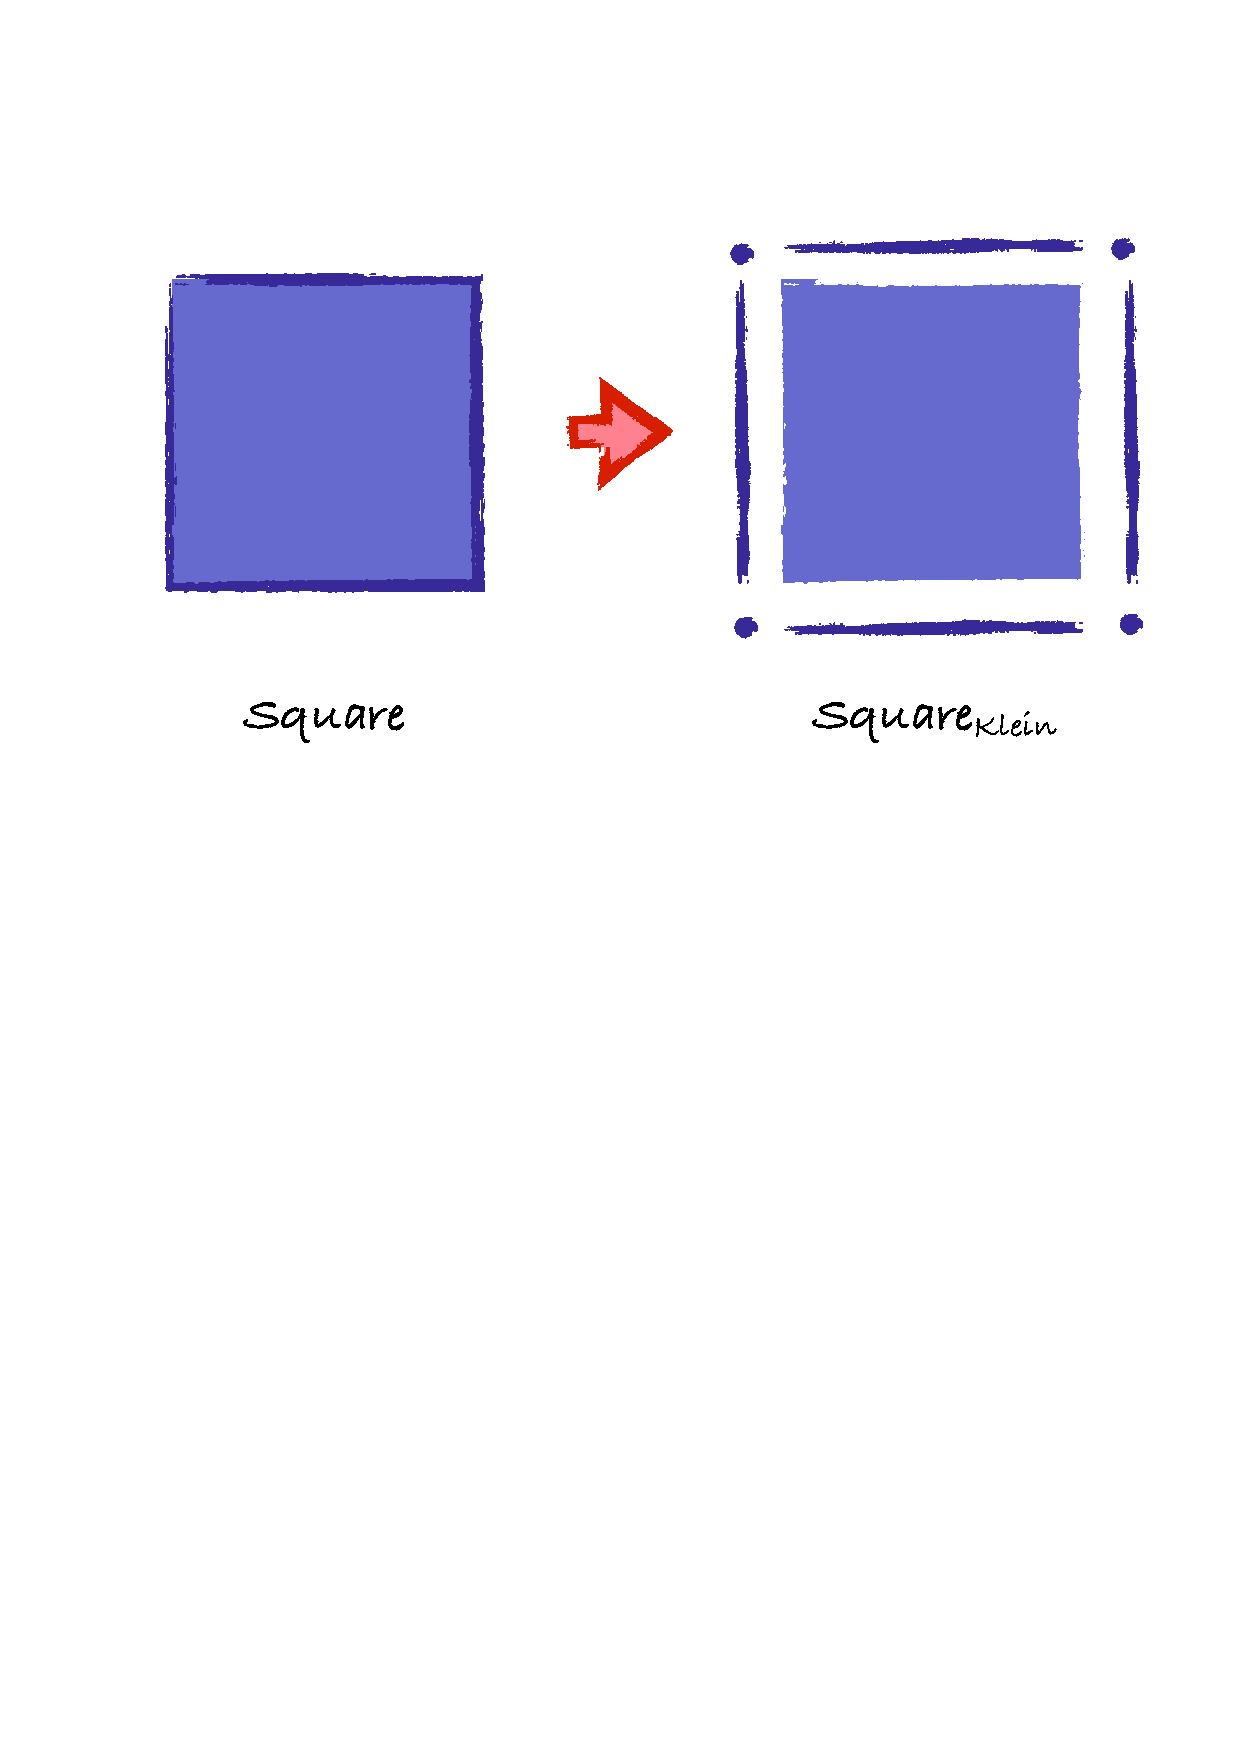
\includegraphics[width=.65\textwidth]{Figures/Square-Klein.pdf}
    \vspace{-\baselineskip}
    \caption{Klein's exploded view of the square.}
    \label{Exploded-view-of-the-square.}
  \end{figure}
  One can also access an aspect of the structure of a diffeological space by means of sum of parts:
  consider the group of diffeomorphisms $\Diff(X)$ a diffeological space $X$.
  It decomposes the space into a set of orbits $\cO \in X/\Diff(X)$.
  Then we reconstruct a finer diffeological space by considering the sum of the orbits,
  an exploded view of the space revealing its singular structure.
  We can call it the Klein's exploded view.
  $$%
    X_{\mathrm{Klein}} = \coprod_{\cO \in X/\Diff(X)} \cO.
    $$%
\end{Article}

%%%%%%%%%%%%%%%%%%%%%%%%%%%%%%%%%%%%%%%%%%%%%%%%%%%%%%%%%%
%%
%% MARK:  Grow and Multiply
%%
%%%%%%%%%%%%%%%%%%%%%%%%%%%%%%%%%%%%%%%%%%%%%%%%%%%%%%%%%%
\section{Grow and multiply}

\begin{Article}{Product diffeology.}
  Consider a family $(X_i)_{i \in \cI}$ of diffeological spaces,
  for any family of indices.
  Let $\Proj_1$ be the first projection of the direct sum of the $X_i$,
  that is
  $$%
    \Proj_1 \colon \coprod_{i \in \cI} X_i \to \cI
    \quad \text{with} \quad
    \Proj_1(i,x) = i.
    $$%
  The product of the $X_i$ is defined as the set of sections of $\Proj_1$,
  that is
  $$%
    \prod_{i \in \cI} X_i = \big\{ x \colon \cI \to \coprod_{i \in \cI} X_i \mid \Proj_1 \circ x = \Id_\cI \big\}
    $$%
  Let $X = \prod_{i \in \cI} X_i$.
  An element $x \in X$ can be denoted as $x = (x_i)_{i \in \cI}$,
  where $x_i = x(i)$.
  The projection $\pi_i$ on the $i$-th factor $X_i$ is defined by
  $$%
    \pi_i(x) = x_i.
    $$%
  \smuline{Proposition.}There exists on the product $X$ a coarsest diffeology such that each projection $\pi_i$ is smooth.
  Equipped with this diffeology,
  $X$ is called the \emph{diffeological product},
  or simply the \emph{product},
  of the $X_i$.
  
  Actually,
  the projections are subductions.
  A parametrization of the product writes $r \mapsto (x_i(r))_{i \in \cI}$,
  where the $x_i$ are plots of the $X_i$.
  
  Now,
  the category \{Diffeology\} is also \uline{closed by product}.
\end{Article}

\begin{Article}{Examples: some diffeological products.}
  The main example here is the power $\RR^n$ which is the product of $n$ copies of $\RR$ equipped with the smooth diffeology.
\end{Article}

A special and remarkable feature of diffeology is that the set of the smooth maps between diffeological spaces carries a natural diffeology:

\begin{Article}{Functional diffeology.}
  Let $X$ and $X'$ be two diffeological spaces.
  There exists on $\Cinfty(X,X')$ a coarsest diffeology such that the \emph{evaluation map}
  $$%
    \Eval \colon \Cinfty(X,X') \times X \to X'
    \quad\text{defined by}\quad
    \Eval(f,x) = f(x),
    $$%
  is smooth.
  Thus diffeology is called the \emph{functional diffeology}.
  
  The plots of that diffeology are the parametrizations $r \mapsto f_r$,
  defined on some domain $U$,
  such that
  $$%
    (r,x) \mapsto f_r(x)
    \quad \text{from} \quad U \times X \quad \text{to} \quad X'
    $$%
  is smooth.
  That means that for every plot $s \mapsto x_s$ in $X$,
  defined on some domain $V$,
  the parametrization $(r,s) \mapsto f_r(x_s)$,
  defined on $U \times V$,
  is a plot of $X'$.
  
  Now,
  let $X$,
  $X'$ and $X''$ be three diffeological spaces.
  Then,
  \begin{enumerate}
    \item The product
    $$%
      \circ(f,g) = g \circ f,
      $$%
    defined on $\Cinfty(X,X') \times \Cinfty(X',X'')$ to $\Cinfty(X,X'')$,
    is smooth.
    
    \item The spaces $\Cinfty(X, \Cinfty( X', X''))$ and $\Cinfty(X \times X', X'')$ are diffeomorphic.
    The diffeomorphism $\pphi$ consists in the game of parenthesis,
    for all $f \in \Cinfty(X, \Cinfty( X', X''))$
    $$%
      \pphi(f) \colon (x,x') \mapsto f(x)(x').
      $$%
  \end{enumerate}
  We say that the category \{Diffeology\} is \emph{Cartesian closed}.
\end{Article}

\vfill
\centerline{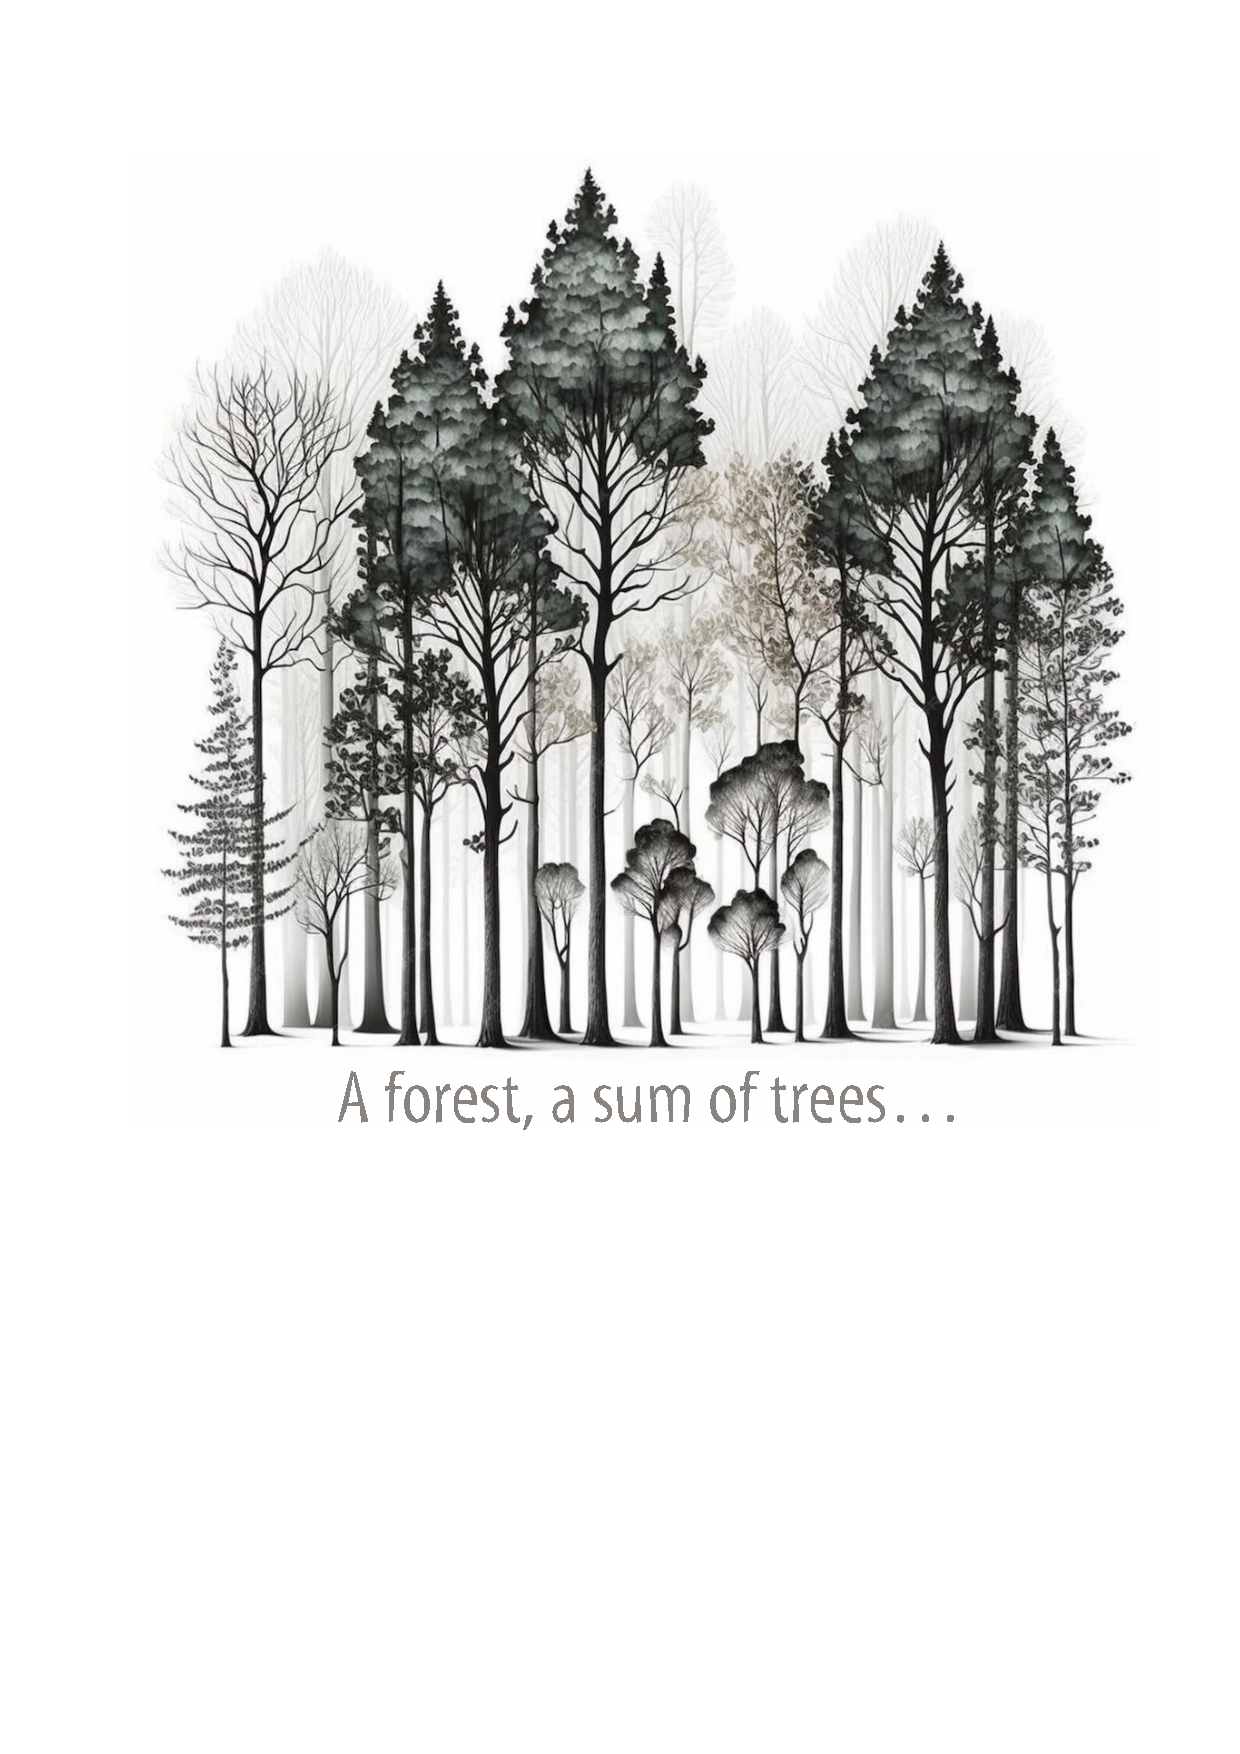
\includegraphics[width=.70\textwidth]{Figures/Trees.pdf}}
